\documentclass[11pt,a4paper]{report}
\usepackage[textwidth=37em,vmargin=30mm]{geometry}
\usepackage{calc,xunicode,amsmath,amssymb,paralist,enumitem,tabu,booktabs,datetime2,xeCJK,xeCJKfntef,listings}
\usepackage{tocloft,fancyhdr,tcolorbox,xcolor,graphicx,eso-pic,xltxtra,xelatexemoji}

\newcommand{\envyear}[0]{2025}
\newcommand{\envdatestr}[0]{2025-07-20}
\newcommand{\envfinaldir}[0]{webdb/2025/20250720/final}

\usepackage[hidelinks]{hyperref}
\hypersetup{
    colorlinks=false,
    pdfpagemode=FullScreen,
    pdftitle={Web Digest - \envdatestr}
}

\setlength{\cftbeforechapskip}{10pt}
\renewcommand{\cftchapfont}{\rmfamily\bfseries\large\raggedright}
\setlength{\cftbeforesecskip}{2pt}
\renewcommand{\cftsecfont}{\sffamily\small\raggedright}

\setdefaultleftmargin{2em}{2em}{1em}{1em}{1em}{1em}

\usepackage{xeCJK,xeCJKfntef}
\xeCJKsetup{PunctStyle=plain,RubberPunctSkip=false,CJKglue=\strut\hskip 0pt plus 0.1em minus 0.05em,CJKecglue=\strut\hskip 0.22em plus 0.2em}
\XeTeXlinebreaklocale "zh"
\XeTeXlinebreakskip = 0pt


\setmainfont{Brygada 1918}
\setromanfont{Brygada 1918}
\setsansfont{IBM Plex Sans}
\setmonofont{JetBrains Mono NL}
\setCJKmainfont{Noto Serif CJK SC}
\setCJKromanfont{Noto Serif CJK SC}
\setCJKsansfont{Noto Sans CJK SC}
\setCJKmonofont{Noto Sans CJK SC}

\setlength{\parindent}{0pt}
\setlength{\parskip}{8pt}
\linespread{1.15}

\lstset{
	basicstyle=\ttfamily\footnotesize,
	numbersep=5pt,
	backgroundcolor=\color{black!5},
	showspaces=false,
	showstringspaces=false,
	showtabs=false,
	tabsize=2,
	captionpos=b,
	breaklines=true,
	breakatwhitespace=true,
	breakautoindent=true,
	linewidth=\textwidth
}






\newcommand{\coverpic}[2]{
    % argv: itemurl, authorname
    Cover photo by #2~~(\href{#1}{#1})
}
\newcommand{\makeheader}[0]{
    \begin{titlepage}
        % \newgeometry{hmargin=15mm,tmargin=21mm,bmargin=12mm}
        \begin{center}
            
            \rmfamily\scshape
            \fontspec{BaskervilleF}
            \fontspec{Old Standard}
            \fontsize{59pt}{70pt}\selectfont
            WEB\hfill DIGEST
            
            \vfill
            % \vskip 30pt
            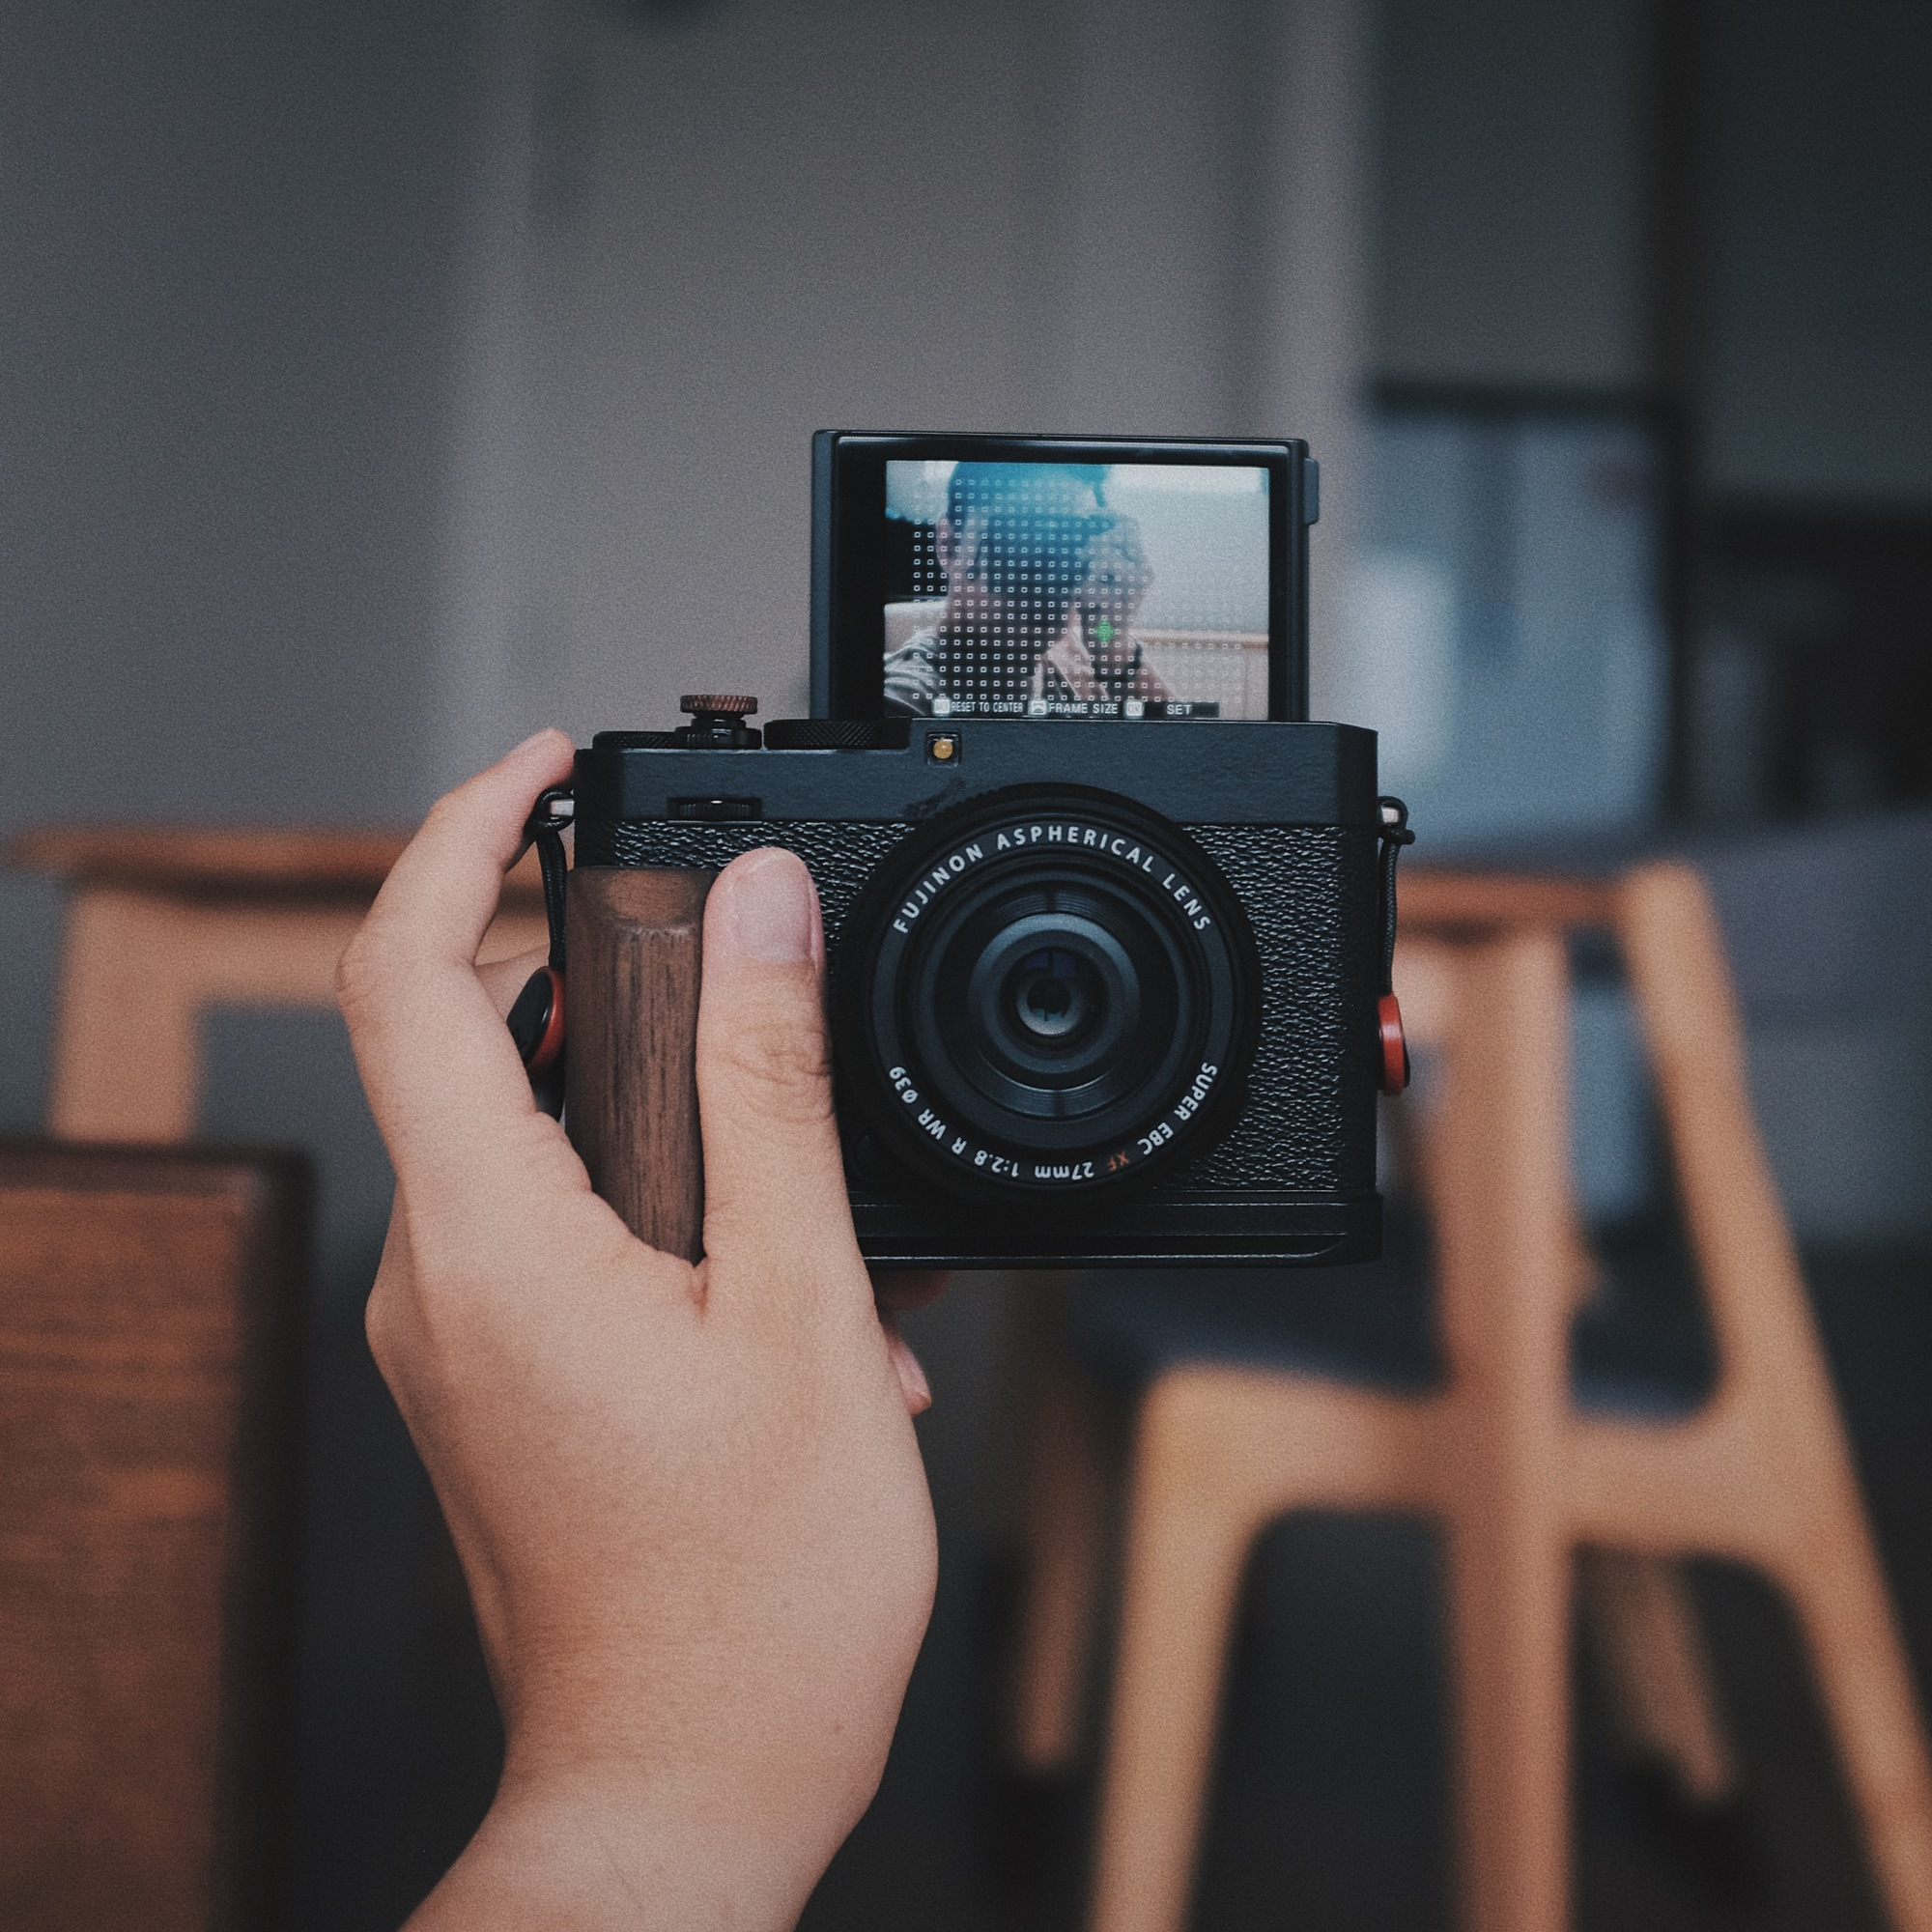
\includegraphics[width=\linewidth]{\envfinaldir/coverpic-prod.jpg}\par
            % \vskip 30pt
            \vfill

            \normalsize\rmfamily\scshape
            \copyright{} The Web Digest Project \hfill\large \envdatestr
        \end{center}
    \end{titlepage}
    % \restoregeometry
}
\newcommand{\simplehref}[1]{%
    \textcolor{blue!80!green}{\href{#1}{#1}}%
}
\renewcommand{\contentsname}{\center\Huge\sffamily\bfseries Contents\par\vskip 20pt}
\newcounter{ipartcounter}
\setcounter{ipartcounter}{0}
\newcommand{\ipart}[1]{
    % \vskip 20pt
    \clearpage
    \stepcounter{ipartcounter}
    \phantomsection
    \addcontentsline{toc}{chapter}{#1}
    % \begin{center}
    %     \Huge
    %     \sffamily\bfseries
    %     #1
    % \end{center}
    % \vskip 20pt plus 7pt
}
\newcounter{ichaptercounter}
\setcounter{ichaptercounter}{0}
\newcommand{\ichapter}[1]{
    % \vskip 20pt
    \clearpage
    \stepcounter{ichaptercounter}
    \phantomsection
    \addcontentsline{toc}{section}{\numberline{\arabic{ichaptercounter}}#1}
    \begin{center}
        \Huge
        \sffamily\bfseries
        #1
    \end{center}
    \vskip 20pt plus 7pt
}
\newcommand{\entrytitlefont}[1]{\subsection*{\raggedright\Large\sffamily\bfseries#1}}
\newcommand{\entryitemGeneric}[2]{
    % argv: title, url
    \parbox{\linewidth}{
        \entrytitlefont{#1}\par\vskip 5pt
        \footnotesize\ttfamily\mdseries
        \simplehref{#2}
    }\vskip 11pt plus 11pt minus 1pt
}
\newcommand{\entryitemGithub}[3]{
    % argv: title, url, desc
    \parbox{\linewidth}{
        \entrytitlefont{#1}\par\vskip 5pt
        \footnotesize\ttfamily\mdseries
        \simplehref{#2}\par\vskip 5pt
        \small\rmfamily\mdseries#3
    }\vskip 11pt plus 11pt minus 1pt
}
\newcommand{\entryitemAp}[3]{
    % argv: title, url, desc
    \parbox{\linewidth}{
        \entrytitlefont{#1}\par\vskip 5pt
        \footnotesize\ttfamily\mdseries
        \simplehref{#2}\par\vskip 5pt
        \small\rmfamily\mdseries#3
    }\vskip 11pt plus 11pt minus 1pt
}
\newcommand{\entryitemHackernews}[3]{
    % argv: title, hnurl, rawurl
    % \parbox{\linewidth}{
    %     \entrytitlefont{#1}\par\vskip 5pt
    %     \footnotesize\ttfamily\mdseries
    %     \simplehref{#3}\par
    %     \textcolor{black!50}{\href{#2}{#2}}
    % }\vskip 11pt plus 11pt minus 1pt
    \begin{minipage}{\linewidth}
            \entrytitlefont{#1}\par\vskip 5pt
            \footnotesize\ttfamily\mdseries
            \simplehref{#3}\par
            \textcolor{black!50}{\href{#2}{#2}}
    \end{minipage}\par\vskip 11pt plus 11pt minus 1pt
}







\begin{document}

\makeheader

\tableofcontents\clearpage




\ipart{Developers}
\ichapter{Hacker News}
\entryitemTwoLinks{TSMC to start building four new plants with 1.4nm technology}{https://news.ycombinator.com/item?id=44618762}{https://www.taipeitimes.com/News/front/archives/2025/07/20/2003840583}

\entryitemTwoLinks{Make Your Own Backup System – Part 1: Strategy Before Scripts}{https://news.ycombinator.com/item?id=44618687}{https://it-notes.dragas.net/2025/07/18/make-your-own-backup-system-part-1-strategy-before-scripts/}

\entryitemTwoLinks{The borrowchecker is what I like the least about Rust}{https://news.ycombinator.com/item?id=44618535}{https://viralinstruction.com/posts/borrowchecker/}

\entryitemTwoLinks{MCP Security Vulnerabilities and Attack Vectors}{https://news.ycombinator.com/item?id=44617910}{https://forgecode.dev/blog/prevent-attacks-on-mcp/}

\entryitemTwoLinks{Rethinking CLI interfaces for AI}{https://news.ycombinator.com/item?id=44617184}{https://www.notcheckmark.com/2025/07/rethinking-cli-interfaces-for-ai/}

\entryitemTwoLinks{It's rude to show AI output to people}{https://news.ycombinator.com/item?id=44617172}{https://distantprovince.by/posts/its-rude-to-show-ai-output-to-people/}

\entryitemTwoLinks{Local LLMs versus offline Wikipedia}{https://news.ycombinator.com/item?id=44617078}{https://evanhahn.com/local-llms-versus-offline-wikipedia/}

\entryitemTwoLinks{Nobody knows how to build with AI yet}{https://news.ycombinator.com/item?id=44616479}{https://worksonmymachine.substack.com/p/nobody-knows-how-to-build-with-ai}

\entryitemTwoLinks{Death by AI}{https://news.ycombinator.com/item?id=44615801}{https://davebarry.substack.com/p/death-by-ai}

\entryitemTwoLinks{Fstrings.wtf}{https://news.ycombinator.com/item?id=44614370}{https://fstrings.wtf/}

\entryitemTwoLinks{I avoid using LLMs as a publisher and writer}{https://news.ycombinator.com/item?id=44614365}{https://lifehacky.net/prompt-0b953c089b44}

\entryitemTwoLinks{Felix Baumgartner, who jumped from stratosphere, dies in Italy}{https://news.ycombinator.com/item?id=44614292}{https://www.theinternational.at/felix-baumgartner-who-jumped-from-stratosphere-dies-in-italy/}

\entryitemTwoLinks{OpenAI claims gold-medal performance at IMO 2025}{https://news.ycombinator.com/item?id=44613840}{https://twitter.com/alexwei\_/status/1946477742855532918}

\entryitemTwoLinks{Linux and Secure Boot certificate expiration}{https://news.ycombinator.com/item?id=44613629}{https://lwn.net/SubscriberLink/1029767/43b62a7a7408c2a9/}

\entryitemTwoLinks{A 14kb page can load much faster than a 15kb page (2022)}{https://news.ycombinator.com/item?id=44613625}{https://endtimes.dev/why-your-website-should-be-under-14kb-in-size/}

\entryitemTwoLinks{YouTube No Translation}{https://news.ycombinator.com/item?id=44613491}{https://addons.mozilla.org/en-US/firefox/addon/youtube-no-translation/}

\entryitemTwoLinks{Pimping My Casio: Part Deux}{https://news.ycombinator.com/item?id=44613486}{https://blog.jgc.org/2025/07/pimping-my-casio-part-deux.html}

\entryitemTwoLinks{Microsoft Office is using an artificially complex XML schema as a lock-in tool}{https://news.ycombinator.com/item?id=44612569}{https://blog.documentfoundation.org/blog/2025/07/18/artificially-complex-xml-schema-as-lock-in-tool/}

\entryitemTwoLinks{Hyatt Hotels are using algorithmic Rest ``smoking detectors''}{https://news.ycombinator.com/item?id=44612487}{https://twitter.com/\_ZachGriff/status/1945959030851035223}

\entryitemTwoLinks{My Self-Hosting Setup}{https://news.ycombinator.com/item?id=44612151}{https://codecaptured.com/blog/my-ultimate-self-hosting-setup/}


\ipart{Developers~~~~(zh-Hans)}
\ichapter{Solidot}
\entryitemGeneric{\hskip 0pt{}英特尔终止了对 Clear Linux 的支持}{https://www.solidot.org/story?sid=81835}

\entryitemGeneric{\hskip 0pt{}苹果起诉通过进入前员工公寓窃取 iOS 26 机密的 YouTube 主播}{https://www.solidot.org/story?sid=81834}

\entryitemGeneric{\hskip 0pt{}狗看电视的模式}{https://www.solidot.org/story?sid=81833}

\entryitemGeneric{\hskip 0pt{}美国法官允许作家对 Anthropic 盗版数百万电子书提起集体诉讼}{https://www.solidot.org/story?sid=81832}

\entryitemGeneric{\hskip 0pt{}Google 起诉 25 名中国籍 BadBox 2.0 运营者}{https://www.solidot.org/story?sid=81831}

\entryitemGeneric{\hskip 0pt{}俄罗斯新法律将搜索``争议内容''定为犯罪行为}{https://www.solidot.org/story?sid=81830}

\entryitemGeneric{\hskip 0pt{}新闻出版业下线绕过付费墙的服务 12ft.io}{https://www.solidot.org/story?sid=81829}

\entryitemGeneric{\hskip 0pt{}Firefox 141 将支持  WebGPU}{https://www.solidot.org/story?sid=81828}

\entryitemGeneric{\hskip 0pt{}预防工作推动发达国家癌症死亡率下降}{https://www.solidot.org/story?sid=81827}

\entryitemGeneric{\hskip 0pt{}智能手机地震预警不比传统地震监测差}{https://www.solidot.org/story?sid=81826}

\entryitemGeneric{\hskip 0pt{}Netflix 制作《刺客信条》真人剧集}{https://www.solidot.org/story?sid=81825}

\entryitemGeneric{\hskip 0pt{}YouTube 主播因演示掌机模拟游戏而面临判刑}{https://www.solidot.org/story?sid=81824}

\entryitemGeneric{\hskip 0pt{}吸烟引起的表观遗传变化与衰老相似}{https://www.solidot.org/story?sid=81823}

\entryitemGeneric{\hskip 0pt{}比亚迪如何赶超特斯拉}{https://www.solidot.org/story?sid=81822}

\entryitemGeneric{\hskip 0pt{}3.6 亿印度巴帝电信用户将能免费使用先进 AI 模型一年}{https://www.solidot.org/story?sid=81821}

\entryitemGeneric{\hskip 0pt{}研究揭示全球精英离岸隐藏财富的模式}{https://www.solidot.org/story?sid=81820}

\entryitemGeneric{\hskip 0pt{}SpaceX 的 Falcon 9 火箭发射了亚马逊的 24 颗宽带卫星}{https://www.solidot.org/story?sid=81819}

\entryitemGeneric{\hskip 0pt{}农业塑料带来的污染挑战}{https://www.solidot.org/story?sid=81818}

\entryitemGeneric{\hskip 0pt{}Google 安全研究员报告 SonicWall 被植入后门}{https://www.solidot.org/story?sid=81817}

\entryitemGeneric{\hskip 0pt{}金平菇入侵北美改变当地菌落}{https://www.solidot.org/story?sid=81816}\ichapter{V2EX}
\entryitemGeneric{\hskip 0pt{}[程序员] 建议开一个 Ai IDE 节点, 专门讨论相关软件工具}{https://www.v2ex.com/t/1146387}

\entryitemGeneric{\hskip 0pt{}[职场话题] 入职后收到更好的 offer 该怎么提离职?}{https://www.v2ex.com/t/1146385}

\entryitemGeneric{\hskip 0pt{}[问与答] 求大佬推荐个好用的 iOS 版 nga 论坛 app}{https://www.v2ex.com/t/1146384}

\entryitemGeneric{\hskip 0pt{}[生活] 12315 举报 抖音 平台 橱窗 搞 sex, 不予立案,还有什么举报方法吗?}{https://www.v2ex.com/t/1146382}

\entryitemGeneric{\hskip 0pt{}[生活] 饿了么 干不过 美团 真的是有道理的!}{https://www.v2ex.com/t/1146381}

\entryitemGeneric{\hskip 0pt{}[iPhone] iPhone 是如何实现钱包刷卡公交记录站点信息的}{https://www.v2ex.com/t/1146379}

\entryitemGeneric{\hskip 0pt{}[汽车] 老司机们,某瓜某帝的二手百公里车能买吗?}{https://www.v2ex.com/t/1146378}

\entryitemGeneric{\hskip 0pt{}[问与答] 刚做完近视手术,我也来聊聊}{https://www.v2ex.com/t/1146377}

\entryitemGeneric{\hskip 0pt{}[分享发现] 有人把 Coldplay 的 Kiss Cam 事件做成了游戏…叫 Coldplay Canoodlers}{https://www.v2ex.com/t/1146376}

\entryitemGeneric{\hskip 0pt{}[Python] PySide6 竟然能开发安卓 APP 了}{https://www.v2ex.com/t/1146375}

\entryitemGeneric{\hskip 0pt{}[宠物] [上海地区接上门喂养] 上门喂猫上门遛狗统统都可以}{https://www.v2ex.com/t/1146374}

\entryitemGeneric{\hskip 0pt{}[生活] 县城的人未必能接受二线城市及以上的物业}{https://www.v2ex.com/t/1146373}

\entryitemGeneric{\hskip 0pt{}[Android] 小白想换个手机,求推荐}{https://www.v2ex.com/t/1146372}

\entryitemGeneric{\hskip 0pt{}[问与答] 最近江苏扬州电信、山东烟台电信似乎很活跃啊,建议站长这些 IP 直接拉黑吧}{https://www.v2ex.com/t/1146369}

\entryitemGeneric{\hskip 0pt{}[宽带症候群] 湖北奠信家宽似乎也有小黑屋了?}{https://www.v2ex.com/t/1146366}

\entryitemGeneric{\hskip 0pt{}[问与答] 稳定币的爆火,会带动 web3 的崛起吗?有没有必要转战 web3 呢}{https://www.v2ex.com/t/1146365}

\entryitemGeneric{\hskip 0pt{}[Chrome] 如何强制 chrome 浏览器使用 QUIC 连接?}{https://www.v2ex.com/t/1146364}

\entryitemGeneric{\hskip 0pt{}[哔哩哔哩] B 站对剧集类内容使用 AI(?)生成 4k 和 HDR 画质}{https://www.v2ex.com/t/1146363}

\entryitemGeneric{\hskip 0pt{}[问与答] Ubuntu 网关 VM 上 dnsmasq 启动失败 (exit code 2),用于 Clash Meta 透明代理 DHCP/DNS 网关}{https://www.v2ex.com/t/1146362}

\entryitemGeneric{\hskip 0pt{}[问与答] windows 只在前台的应用播放声音,有这样的软件吗}{https://www.v2ex.com/t/1146361}

\entryitemGeneric{\hskip 0pt{}[YouTube] 油管为什么不给我流量?}{https://www.v2ex.com/t/1146360}

\entryitemGeneric{\hskip 0pt{}[分享发现] n8n 的基础安装分享}{https://www.v2ex.com/t/1146359}

\entryitemGeneric{\hskip 0pt{}[Cursor] cursor pro 的用量太模糊了,到底能用多少量?开了个两个账号,一个用到 \$165 才限制 一个\$55}{https://www.v2ex.com/t/1146357}

\entryitemGeneric{\hskip 0pt{}[信息安全] 微信 3.9 版本暴 RCE 漏洞}{https://www.v2ex.com/t/1146356}

\entryitemGeneric{\hskip 0pt{}[Mac mini] 无痛从 MBP 切换至 Mac-mini 了~}{https://www.v2ex.com/t/1146355}

\entryitemGeneric{\hskip 0pt{}[程序员] 项目自荐: GPT-Load - 高性能 AI 网关,为多种大模型服务提供统一的负载均衡和密钥管理。}{https://www.v2ex.com/t/1146354}

\entryitemGeneric{\hskip 0pt{}[分享发现] 今天被一包杂牌薯片征服了,墙裂推荐!}{https://www.v2ex.com/t/1146353}

\entryitemGeneric{\hskip 0pt{}[问与答] 在全民所有制中,如果按照现代产权原理,全民所有的财产有我的一份,那我转国籍的时候,政府是否愿意把我应得的一份退还给我带走呢?}{https://www.v2ex.com/t/1146351}

\entryitemGeneric{\hskip 0pt{}[问与答] 移动宽带光猫改桥接会限速?}{https://www.v2ex.com/t/1146350}

\entryitemGeneric{\hskip 0pt{}[问与答] 求推荐电动滑板车,用于通勤使用}{https://www.v2ex.com/t/1146349}

\entryitemGeneric{\hskip 0pt{}[远程工作] 包网项目招 golang 开发}{https://www.v2ex.com/t/1146348}

\entryitemGeneric{\hskip 0pt{}[问与答] 想买一双索康尼胜利 23,请问大家在哪里买便宜一些?}{https://www.v2ex.com/t/1146347}

\entryitemGeneric{\hskip 0pt{}[分享发现] 偶然发现 cctv 下的 oss 被用来涉黄,怪不得之前阿里云被封呢}{https://www.v2ex.com/t/1146346}

\entryitemGeneric{\hskip 0pt{}[分享发现] 坚果云? jianguoy?}{https://www.v2ex.com/t/1146345}

\entryitemGeneric{\hskip 0pt{}[分享创造] 开源一个带页面标题和链接信息的二维码卡片生成器,欢迎试用和反馈}{https://www.v2ex.com/t/1146343}

\entryitemGeneric{\hskip 0pt{}[职场话题] 为什么你的领导总说你「沟通有问题」?}{https://www.v2ex.com/t/1146342}

\entryitemGeneric{\hskip 0pt{}[分享发现] 香港 ClubSIM 关闭 eSIM 申请 和 下架欧洲流量}{https://www.v2ex.com/t/1146341}

\entryitemGeneric{\hskip 0pt{}[问与答] AIGC 对内容社区和 UGC 类的平台,是好是坏?}{https://www.v2ex.com/t/1146340}

\entryitemGeneric{\hskip 0pt{}[路由器] 求推荐分布式路由器}{https://www.v2ex.com/t/1146339}

\entryitemGeneric{\hskip 0pt{}[VXNA] 申请收录个人博客 https://blog.irain.in}{https://www.v2ex.com/t/1146338}

\entryitemGeneric{\hskip 0pt{}[问与答] 有没有快速独立站建站的项目?}{https://www.v2ex.com/t/1146337}

\entryitemGeneric{\hskip 0pt{}[NAS] 机械硬盘, 10 万次启停,居然健康 100\%}{https://www.v2ex.com/t/1146334}

\entryitemGeneric{\hskip 0pt{}[程序员] 想了解一下大家对 Markdown 协同编辑工具的使用情况和痛点}{https://www.v2ex.com/t/1146333}

\entryitemGeneric{\hskip 0pt{}[问与答] 周末上 V2EX 刷贴的是不是都是加班的 v 油}{https://www.v2ex.com/t/1146332}

\entryitemGeneric{\hskip 0pt{}[问与答] 有什么好的副屏显示器推荐的吗?}{https://www.v2ex.com/t/1146331}

\entryitemGeneric{\hskip 0pt{}[Go 编程语言] 请教个关于 go 开发游戏服务端的问题}{https://www.v2ex.com/t/1146330}

\entryitemGeneric{\hskip 0pt{}[分享创造] 耗时一周,我的编程语言 Hulo 新增 Bash 转译和包管理工具}{https://www.v2ex.com/t/1146328}

\entryitemGeneric{\hskip 0pt{}[Cloudflare] Cloudflare Free CDN 都被解析到末尾为 1 的 IP,还有什么办法能救回来么?}{https://www.v2ex.com/t/1146327}

\entryitemGeneric{\hskip 0pt{}[DNS] 在国内买了域名转移到了 NAME 域名商,解析还是污染,还有救吗?}{https://www.v2ex.com/t/1146325}

\entryitemGeneric{\hskip 0pt{}[问与答] 微软 E5 账号续订 身份验证方法策略要在 9 月 30 日前迁移完成是否对续订有影响?}{https://www.v2ex.com/t/1146324}


\ipart{Generic News}







\clearpage
\leavevmode\vfill
\footnotesize

Copyright \copyright{} 2023-2025 Neruthes and other contributors.

This document is published with CC BY-NC-ND 4.0 license.

The entries listed in this newsletter may be copyrighted by their respective creators.

This newsletter is generated by the Web Digest project.

The newsletters are also delivered via Telegram channel \CJKunderline{\href{https://t.me/webdigestchannel}{https://t.me/webdigestchannel}}.\\
RSS feed is available at \CJKunderline{\href{https://webdigest.pages.dev/rss.xml}{https://webdigest.pages.dev/rss.xml}}.

This newsletter is available in PDF at
\CJKunderline{\href{https://webdigest.pages.dev/}{https://webdigest.pages.dev/}}.

The source code being used to generate this newsletter is available at\\
\CJKunderline{\href{https://github.com/neruthes/webdigest}{https://github.com/neruthes/webdigest}}.

This newsletter is also available in
\CJKunderline{\href{http://webdigest.pages.dev/readhtml/\envyear/WebDigest-20250720.html}{HTML}} and
\CJKunderline{\href{https://github.com/neruthes/webdigest/blob/master/markdown/\envyear/WebDigest-20250720.md}{Markdown}}.


\coverpic{https://unsplash.com/photos/snowy-mountains-under-a-colorful-twilight-sky-kE1zeGSBJJk}{Marek Piwnicki}


\end{document}
